%----------------------------------------------------------------------------
\chapter{Megvalósítás}\label{sect:megvalositas}
%----------------------------------------------------------------------------

A megvalósítás során csak az \textbf{objektumorientált programozás} (object-oriented programming -- OOP) merült fel mint felhasználható módszertan. Az általánosan elterjedt koncepció lehetővé teszi egy komplex probléma kellően intuitív megfogalmazását és átlátható leírását. Erre a fejlesztés során szükség is volt, hiszen a meglehetősen összetetté váló programot csak gondos tervezéssel és kivitelezéssel lehetett megfelelő minőségben előállítani.

Az alkalmazás fejlesztését tehát az OOP paradigmáinak szem előtt tartásával végeztem. Az ismert alapelvek néhány szóban:

\begin{itemize}
  \item \textbf{absztrakció (abstraction):} a probléma valós világbeli objektumok mintájára történő modellezése, a lényegtelen részletek elhagyásával, a lényeges tulajdonságok kiemelésével
  \item \textbf{egységbe zárás (encapsulation):} az egyes osztályok és objektumpéldányok saját maguk rendelkezzenek a futások során szükséges adatok és metódusok felett
  \item \textbf{öröklődés (inheritance):} lehetséges egy általános ősosztály tetszőleges kiegészítése, specializálása a közös elemek megtartásával
  \item \textbf{polimorfizmus (polymorphism):} az egyes műveleteket képesek legyünk bemeneti paraméterek széles skáláján végrehajtani (metódus- vagy operátor-felüldefiniálás)
\end{itemize}

\bigskip

\texttt{+++ melyik szakaszban mi van +++}

%,,,,,,,,,,,,,,,,,,,,,,,,,,,,,,,,,,,,,,,,,,,,,,,,,,,,,,,,,,,,,,,,,,,,,,,,,,,,
\section{Követelmények}\label{sect:kovetelmenyek}
%,,,,,,,,,,,,,,,,,,,,,,,,,,,,,,,,,,,,,,,,,,,,,,,,,,,,,,,,,,,,,,,,,,,,,,,,,,,,

Mielőtt a fejezet későbbi szakaszaiban részletekbe menőben bemutatom az elkészült alkalmazás architektúráját, illetve osztályainak pontos működését, szeretném dokumentálni a kész programra vonatkozó \textbf{követelményeket, azaz specifikációt}.

\bigskip

Az alkalmazás legyen képes:

\begin{itemize}
  \item valósidejű \textbf{videofolyamot} olvasni a számítógépre kötött webkameráról (lásd \sectref{infracam} szakasz)
  \item a videofolyam feldolgozásával a \textbf{pupillapozíció meghatározására} a \sectref{pupillakov} szakaszban leírtak szerint.
  \item a tekintet \textbf{kalibrációjára} a \sectref{kalibracio} szakaszban ismertetett módszer felhasználásával.
  \item \textbf{munkamenetek} (session) rögzítésére a képernyő tartalmának mentésével együtt.
  \item a korábbi munkamenetek listázására, rendezésére, törlésére.
  \item munkamenetek \textbf{visszajátszására}.
  \item a munkamenetek alapján \textbf{hőtérképek} generálására (lásd \sectref{web} szakasz)
\end{itemize}

%,,,,,,,,,,,,,,,,,,,,,,,,,,,,,,,,,,,,,,,,,,,,,,,,,,,,,,,,,,,,,,,,,,,,,,,,,,,,
\section{Architektúra}\label{sect:architektura}
%,,,,,,,,,,,,,,,,,,,,,,,,,,,,,,,,,,,,,,,,,,,,,,,,,,,,,,,,,,,,,,,,,,,,,,,,,,,,
  
  Az implementációt a \sectref{technologia} fejezetben bemutatott technológiák (OpenCV, Qt, Qt Creator) felhasználásával \textbf{C++ nyelven készítettem el}. A kialakított osztályhierarchia a \figref{overview} ábrán látható módon épül fel. A kibővített osztálydiagram  -- a fontos változók és funkciók feltüntetésével -- megtalálható az \sectref{osztalydiagram} függelékben.

\begin{figure}[!ht]
\centering
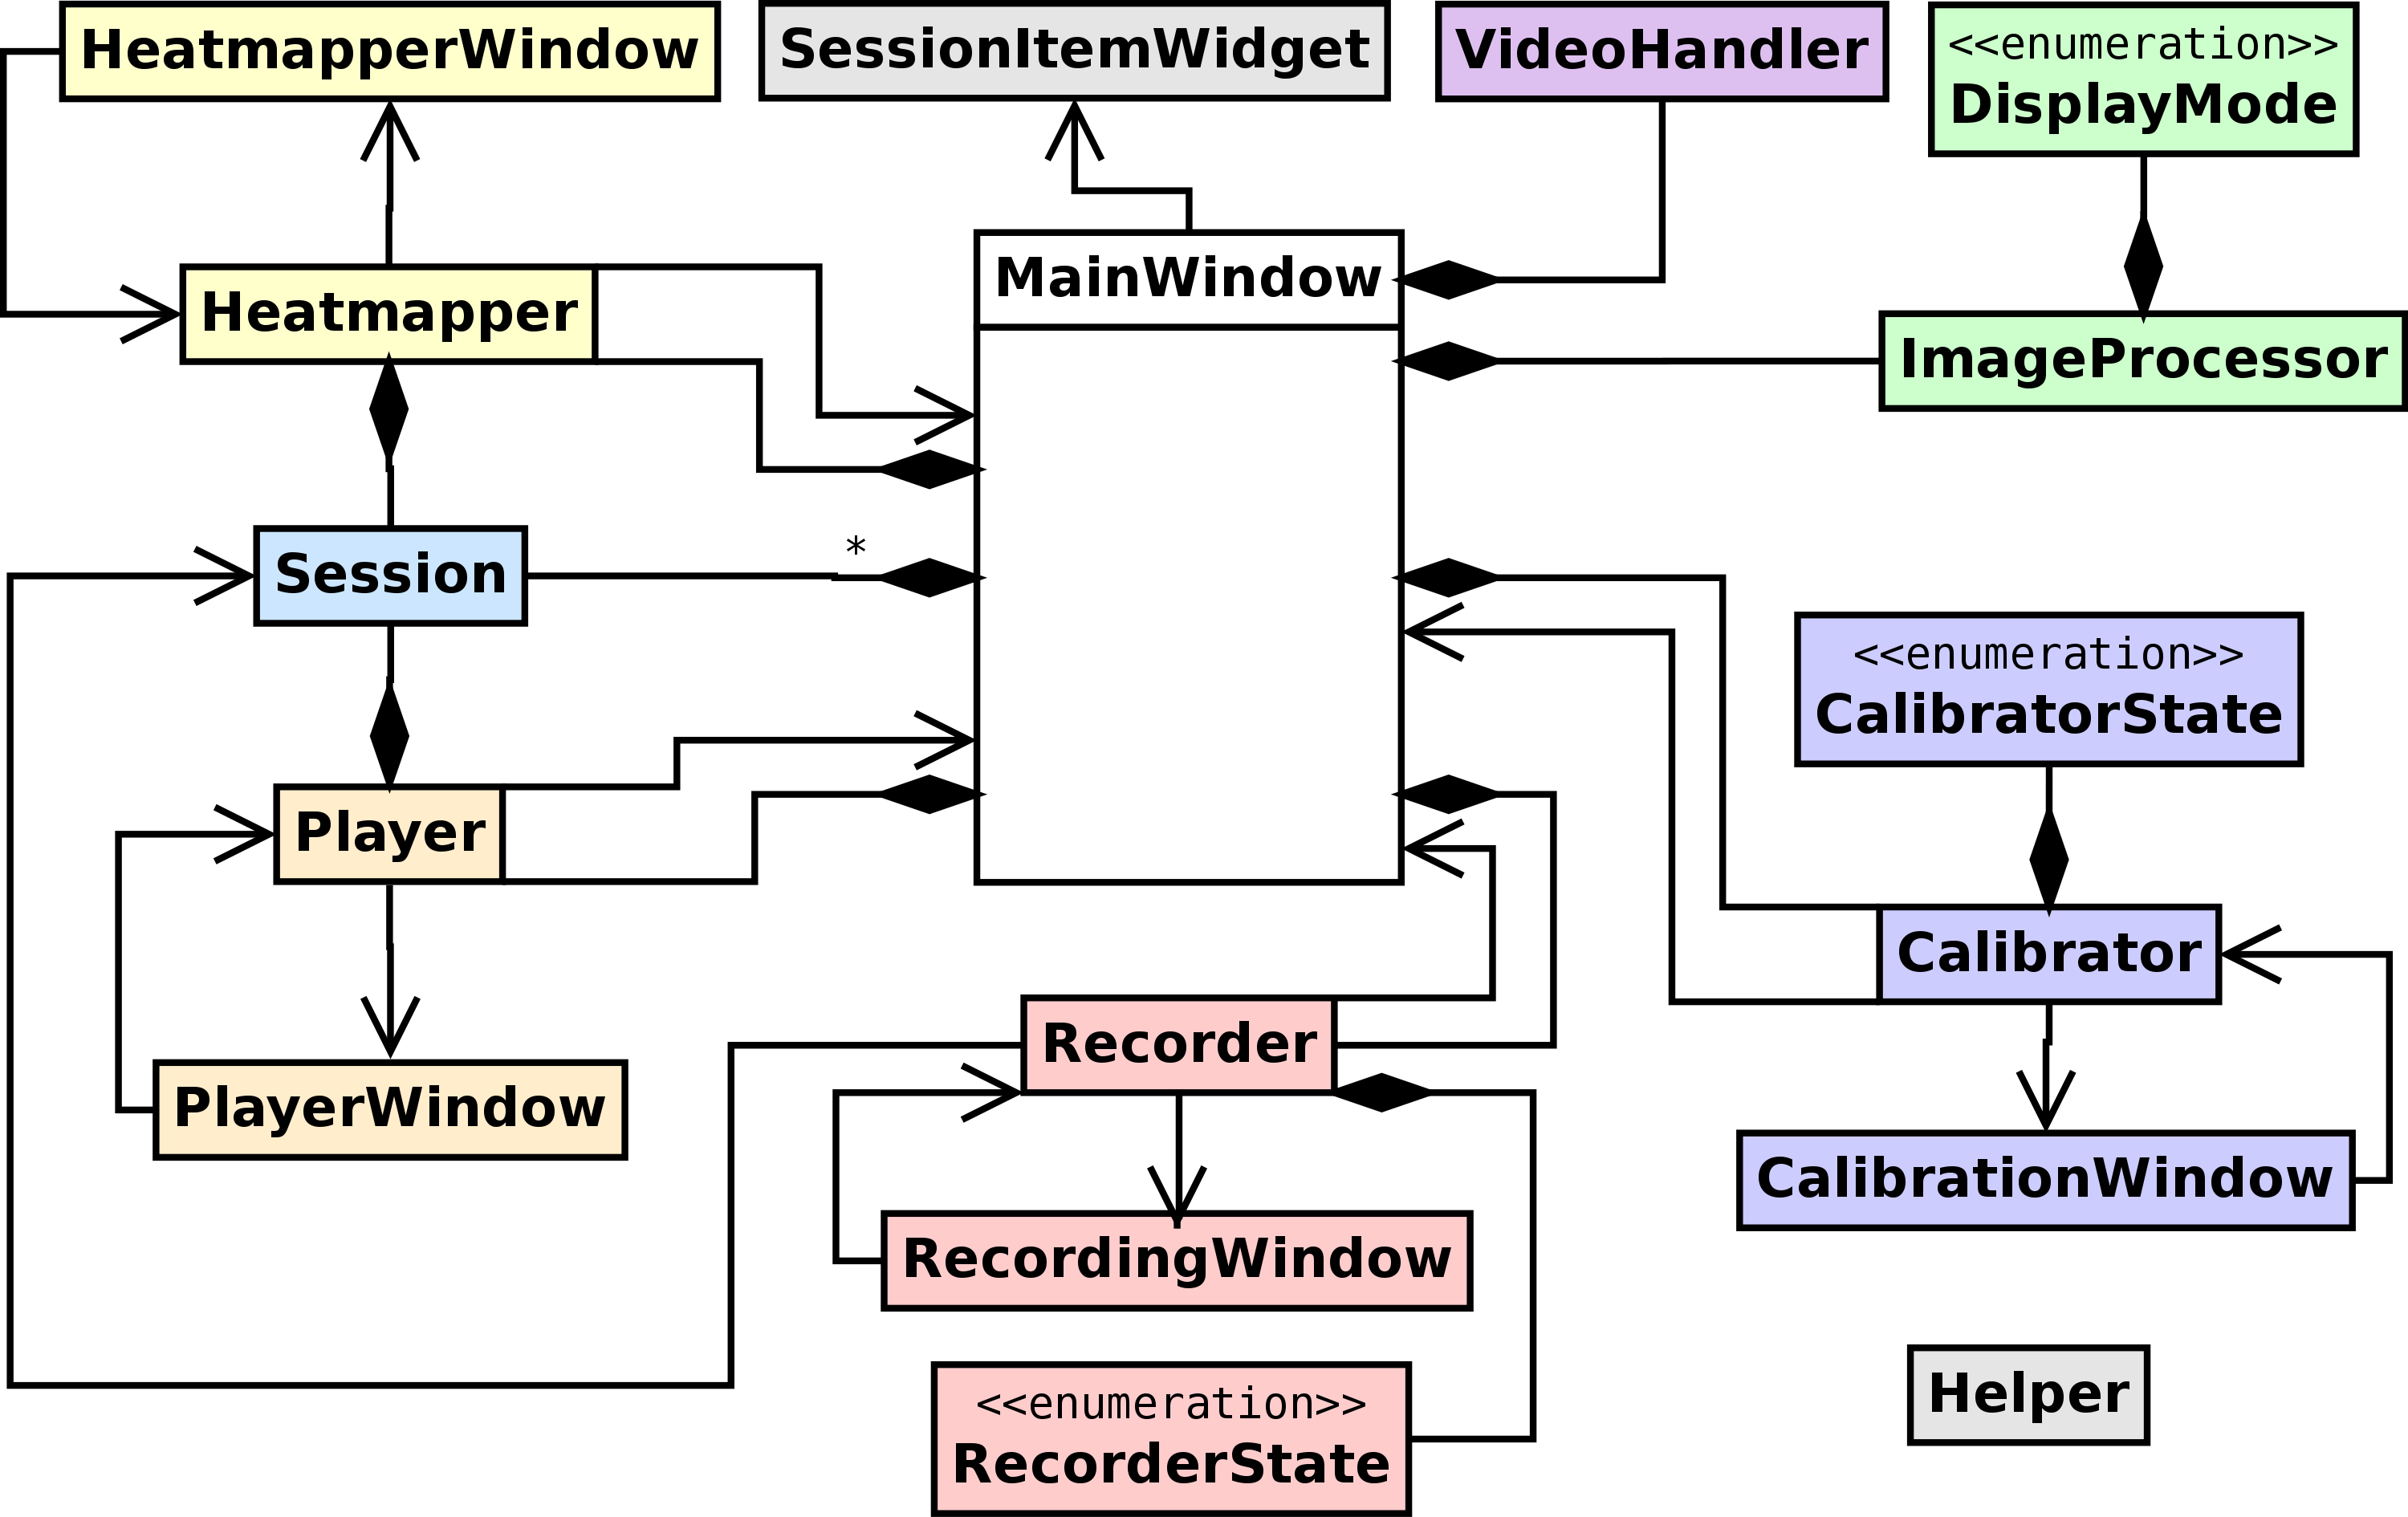
\includegraphics[width=140mm, keepaspectratio]{figures/overview_aa.png}
\caption{Az alkalmazás osztályhierarchiája}
\label{fig:overview}
\end{figure}

Az ábrákon színkódokkal jelöltem a logikailag összetartozó osztályokat. Az alkalmazás egyes funkcióit a videofolyam feldolgozásától a rögzített felvételek visszajátszásáig osztályok egy-egy csoportja végzi

%............................................................................
\subsection{A \texttt{MainWindow} osztály}\label{sect:mainwindow}
%............................................................................

blabla

%............................................................................
\subsection{A \texttt{VideoHandler} osztály}\label{sect:videohandler}
%............................................................................

blabla

%............................................................................
\subsection{Az \texttt{ImageProcessor} osztály}\label{sect:imageprocessor}
%............................................................................

blabla

%............................................................................
\subsection{A \texttt{Calibrator} osztály}\label{sect:calibrator}
%............................................................................

blabla

%............................................................................
\subsection{A \texttt{Session} osztály}\label{sect:session}
%............................................................................

blabla

%............................................................................
\subsection{A \texttt{Recorder} osztály}\label{sect:recorder}
%............................................................................

blabla

%............................................................................
\subsection{A \texttt{Player} osztály}\label{sect:player}
%............................................................................

blabla

%............................................................................
\subsection{A \texttt{Heatmapper} osztály}\label{sect:heatmapper}
%............................................................................

blabla

%,,,,,,,,,,,,,,,,,,,,,,,,,,,,,,,,,,,,,,,,,,,,,,,,,,,,,,,,,,,,,,,,,,,,,,,,,,,,
\section{Felhasználói felület}\label{sect:gui}
%,,,,,,,,,,,,,,,,,,,,,,,,,,,,,,,,,,,,,,,,,,,,,,,,,,,,,,,,,,,,,,,,,,,,,,,,,,,,

\texttt{+++ leiras + kepek a felhasznalo feluletrol +++}

%,,,,,,,,,,,,,,,,,,,,,,,,,,,,,,,,,,,,,,,,,,,,,,,,,,,,,,,,,,,,,,,,,,,,,,,,,,,,
\section{Felhasználói dokumentáció}\label{sect:docs}
%,,,,,,,,,,,,,,,,,,,,,,,,,,,,,,,,,,,,,,,,,,,,,,,,,,,,,,,,,,,,,,,,,,,,,,,,,,,,

\texttt{+++ az alkalmazas pontos hasznalata (tobb monitor, stb) +++}

%,,,,,,,,,,,,,,,,,,,,,,,,,,,,,,,,,,,,,,,,,,,,,,,,,,,,,,,,,,,,,,,,,,,,,,,,,,,,
\section{Tesztelés, eredmények}\label{sect:teszteles}
%,,,,,,,,,,,,,,,,,,,,,,,,,,,,,,,,,,,,,,,,,,,,,,,,,,,,,,,,,,,,,,,,,,,,,,,,,,,,

\texttt{+++ tesztelesi dokumentacio (ide mit?) +++}